\section{ExtRA Framework}
\label{sec:method}

\begin{figure*}[th]
	\centering
	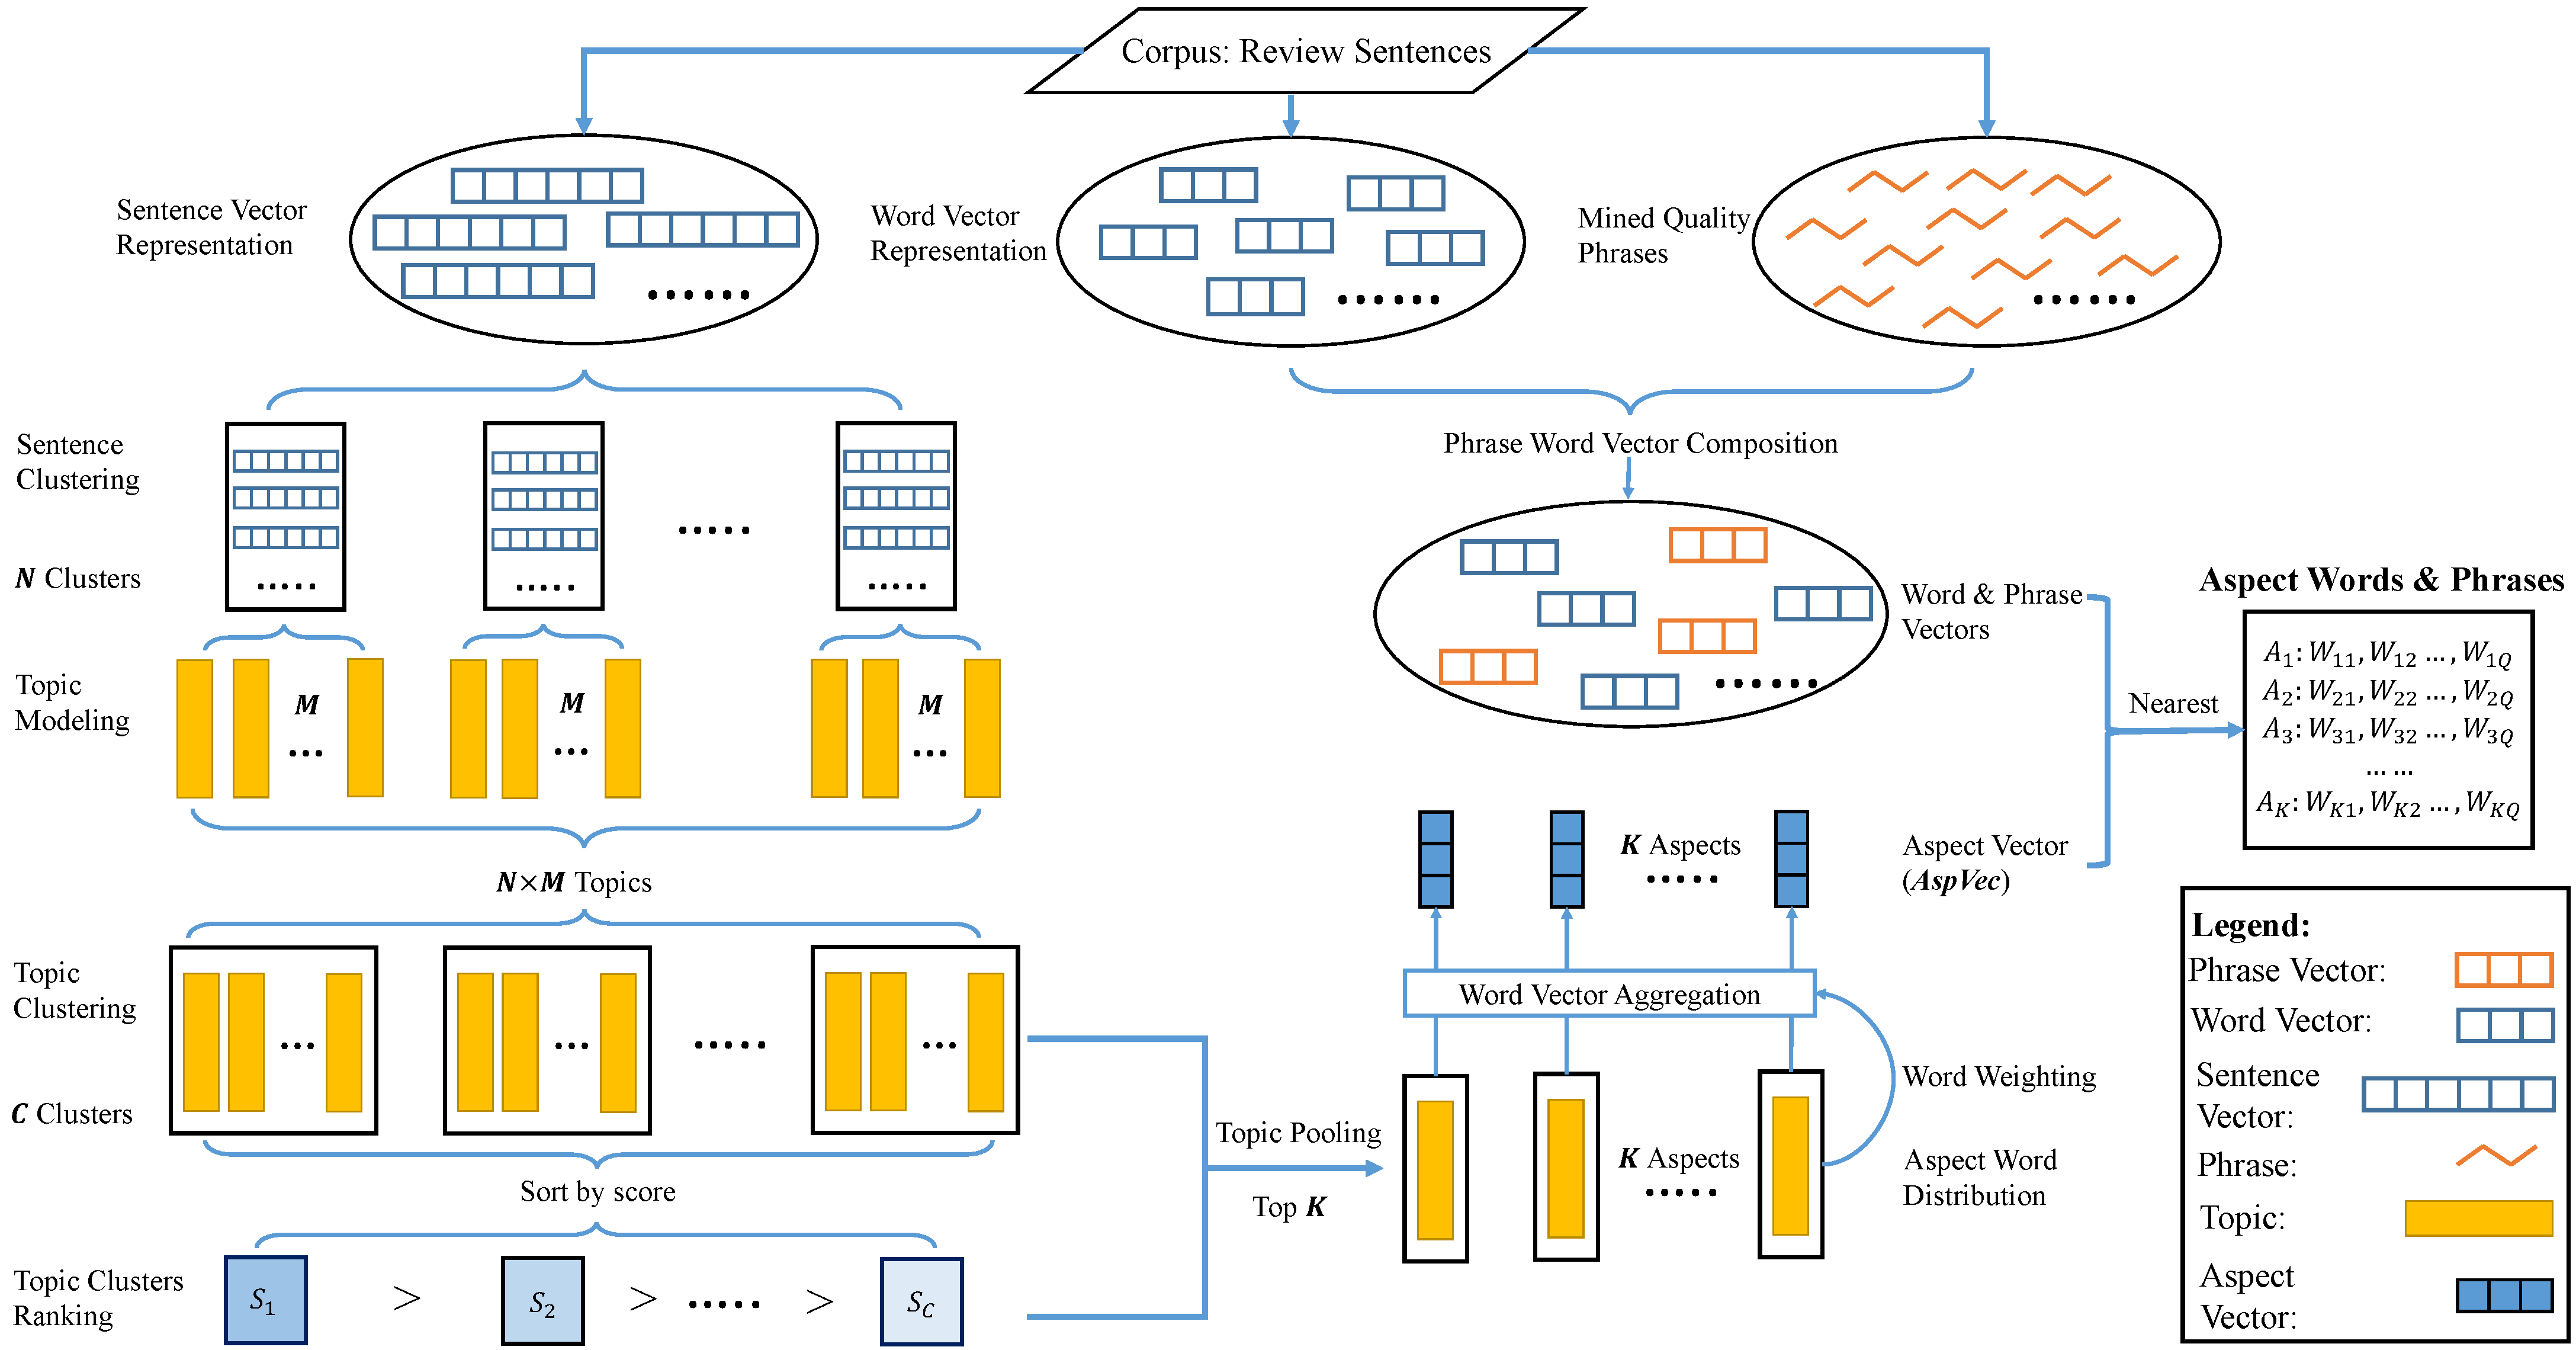
\includegraphics[width=\textwidth]{figures/overview}
	\caption{Our overall framework.}
	\label{fig:framework}
\end{figure*}
In this section, we first state the \textit{review aspect extraction problem}, then present the overall workflow of ExtRA, and finally talk about the framework stage by stage. 
\subsection{Problem Statement}
The review aspect extraction problem is how to extract a certain number of words (or phrases) 
from customer reviews about a given type of product,
each of which represents a prominent and distinct review aspect. 

For instance, if the given product type is \textit{hotel}, we expect a successful extraction framework to extract the aspect terms as follows: 
\textit{room, location, staff, breakfast, pool, etc.}
%Here $K$ is an constant parameter for the problem. 
%The set of reviews and the number of aspects are inputs.
%Note that in this definition we don't use cross-domain information, 
%that is, for one product type we only use the reviews of that domain.
%Thus, our model can extract aspects across domains with ease.
%This allows us to apply the model to any domain with ease.
\subsection{Overall Workflow}
The overall workflow of ExtRA framework is shown in \figref{fig:framework}, \ZY{which consists of a preprocessing step plus 5 stages}:
% Sentence Representations and Clustering
\begin{enumerate}
\item\textit{\ZY{Preprocessing: Derive Synonyms from Wikipedia.}}
\ZY{We derive those mentions of noun words and mined phrases which have the common transitive target concept as a synonym. Then We substitute the mention to its corresponding synonym in the preprocessing step. }

\item\textit{Sentence Representations and Clustering.} 
We encode review sentences into distributed representations, and then cluster them into several coarse-grained topics in an unsupervised way.
%Topic Modeling
\item \textit{Topic Modeling for Each Sentence Cluster.} 
In order to obtain potential prominent aspect topics, 
we perform the topic modeling in each sentence cluster. 
We do this in each cluster instead of all sentences because
topic modeling tends to be more accurate on a smaller and
relatively cleaner corpus.
Also, we treat each sentence cluster equally, so that topic modeling 
process is less affected by uneven distribution of aspects in
user reviews.
% Topic Clustering
\item \textit{Topic Clustering.} To improve the consistency of the 
topics in each sentence cluster, we further cluster the topics from 
all sentence clusters to obtain the final purified topic clusters. 
This step isolates away noisy topics by redistributing the 
potential topics in the process of clustering.
% Aspect Cluster Ranking
\item  \textit{Topic Cluster Ranking.} We select the most prominent 
and distinct topic clusters by a ranking mechanism.
% Aspect Generation
\item \textit{Aspect Extraction from Ranked Topic Clusters.} 
In the final stage, we extract aspect terms from previously ranked topic clusters. 
We first propose a word-ranking based method, which can score each candidate term for its prominence. 
For extracting the aspect phrases, we further propose an encoding method.
It represents each selected topic cluster with a vector,  so that we can extract  the most prominent aspect terms and phrases
based on nearest neighbors searching in 
a shared vector space.  
\end{enumerate}
Next we will discuss each stage in more details.
%\BL{we can briefly introduce the 5 stages here in the preamble}

\subsection{Stage 0: Preprocessing: Derive Synonyms from Wikipedia}
\ZY{
	Wikipedia article names are very good world concepts constructed by human efforts. We use the Wikipedia ontology to aggregate those terms with similar semantics but different mentions in the reviews as synonyms, such as {\em front desk} and {\em receptionist}.
	First, we use AutoPharse to mine high quality bi-gram phrases out of the review texts. 
	We substitute those mentions of noun words and mined phrases which are redirected concepts in Wikipedia to their transitive target concepts by leveraging redirect links.
	After such preprocessing step, we reduce the number of distinct concepts in our reivew texts, which is the great benefit of learning embeddings in the following stage.
}

\subsection{Stage 1: Sentence Representations and Clustering}
Consider the following hotel review example:

\begin{quote}
	\textit{\underline{Pool} is small and only 4 ft but refreshing. \underline{Hot tub} also there. \underline{Staff} were super friendly each day. \underline{Room} was nothing special but clean and comfy. Lots of \underline{restaurants and bars} nearby. \underline{Breakfast} was great and despite being a busy weekend there was always a big selection available.''}
\end{quote}

%For user reviews, many topics can be compressed into a short paragraph and
%each topic corresponds to a potential aspect of the product.
%A typical hotel review extracted from 
%is shown below. 
From this example,
we can conclude that topics (underlined) in reviews can shift very quickly, and
adjacent sentences may refer to 
completely different aspects about a product. 
%Plus, sentences about the same review aspect may not 
%appear consecutively in a review. 
%we convert each sentence in the reviews into a vector representation 
%and cluster them in to $N$ clusters of semantically similar sentences.
Such fine-grained semantic shifts in user reviews 
make it more suitable to consider the sentence as our base unit instead of a whole review document. 

Motivated by this observation, we divide all review documents into sentences and then perform sentence clustering.  
Instead of using simplistic methods like bag-of-word representation, 
we leverage distributed representation which encodes words and sentences as low-dimensional real-valued vectors.
Existing sentence embedding methods include averaging word vectors in a sentence, ParagraphVector (PV)\cite{le2014distributed}, LSTM-based methods\cite{hochreiter1997long}, etc.
%Our experiments show that PV performs the best.
After obtaining sentence representations,
we cluster them into $N$ clusters by k-means algorithm\cite{kmeans}.
%We then collect the similar sentences from a review and
%each review document is divided into several shorter documents, each belonging
%to one of the $N$ clusters. 
As a result, we obtain $N$ clusters of sentences each carrying
some coarse-grained semantics.

\subsection{Stage 2: Topic Modeling for Each Sentence Cluster}

%To isolate the noises that exist in the sentence cluster,
%for each sentence cluster we further generate $M$ 
%topics, resulting in $N\times M$ different word distributions in total.
%Sentence clustering step clustered semantical similar sentences together. 
%However, each cluster may still mix up with multiple aspects. 
Although we performed sentence clustering based on 
semantic sentence representations, there still exits some 
sentences that carry multiple topics or contain noise.
For example, the following two sentences are taken from two 
TripAdvisor reviews:
\begin{itemize}
	\item Sentence 1: \textit{``The room was clean, the staff were 
friendly, and I would say the price is very reasonable given the 
proximity to business and leisure destinations around downtown.''}
	
	\item Sentence 2: \textit{``There is a restaurant just 5 min 
walk away with nice Italian food, pizza was great.''}
\end{itemize}
Sentence 1 mentions multiple aspects such as {\em room}, {\em staff} and {\em price};
sentence 2 is mainly about the {\em location} aspect of the hotel
but it contains some irrelevant information  about the food outside
the hotel.
%Thus, it is also difficult for sentence representations like PV to correctly determine the aspects in these sentences. 
%As a result, each cluster contains multiple aspects and there are also overlapping across clusters. 
 
%Fengshi: The result is overlaps between clusters about 
%different aspects and noises within each cluster.

To address such challenges,
we apply topic modeling within each sentence cluster and obtain $M$ topics for each cluster. 
This gives us in total $N\times M$ topics.
Each topic here can be considered as a word distribution.

We choose to use Biterm Topic Model (BTM) \cite{cheng2014btm} for the topic modeling.
It is a word co-occurrence based topic model that learns topics by modeling word-word co-occurrences patterns (i.e., biterms). 
%\KZ{Give the intuition why biterm is a better model than term-document
%model?}
A bi-term consists of two words co-occurring in the same context, for example, in the same short text window.
%On the contrary, LDA \BL{cite} and PLSA \BL{cite} are word-document co-occurrence topic models. 
Unlike word-document co-occurrence based topic modeling methods (such as LDA \cite{Blei2003LatentDA} and PLSA \cite{Hofmann1999ProbabilisticLS,Hofmann2001UnsupervisedLB}), 
BTM models the bi-term occurrences in a corpus, which alleviates the data sparsity problem of short documents.
Therefore, BTM is much more suitable for modeling topics from our review sentence clusters.

%In generation procedure, a biterm is generated by drawn two words independently from a same topic. In other words, the distribution of a biterm $b=(w_i,w_j)$ is defined as:
%\begin{equation}
%	P(b) = \sum_z{P(w_i|z)*P(w_j|z)*P(z)}.
%\end{equation}
%\KZ{What does $k$ mean? The above equation is not right!}
%With Gibbs sampling algorithm, we can learn topics by estimate $P(w|z)$ and $P(z)$.

\tabref{table:overlap} shows an example of topics modeled from hotel reviews ($N=3$  and $M=5$).
%and illustrates the overlap problem.
In this example, there are five topics ($t_1$-$t_5$) extracted from each sentence cluster. 
We find that the core aspects for these 
three clusters should be {\em room}, {\em location} and {\em price} 
respectively.

However, there are still some noise in such sentence clusters:
boldfaced topics are obviously irrelevant to the core aspect of their clusters.  
Especially, ``t5'' in ``Sentence cluster 3'' consists of multiple different aspects.
%Thus, we have to do the next stage for 
%This topic modeling extracts multiple topics from each cluster, and each topic indicates the potential expected aspect.

\begin{table}[t]
	\small
	\centering
	\caption{Topics extracted from three sentence clusters of hotel review.}
	\label{table:overlap}
	\begin{tabular}{|c|l|}
		\hline
		& t1: room bed bedroom size floor \\
		Sentence
		&t2:  bedroom room wall size decor \\
		cluster 1
		&t3:  room bathroom shower water towel \\
		&t4:  room suite size view floor \\
		&t5:  room shower area kitchen bed \\\hline
		
		&t1:  station minute tube location bus \\
		Sentence
		&t2:  location price night place rate\\
		cluster 2
		&t3:  location square station street subway\\
		&t4:  distance bus subway downtown shopping\\
		&t5:  \textbf{restaurant} \textbf{city} \textbf{food} \textbf{buffet} \textbf{place} \\\hline
		
		&t1:  price rate service money star\\
		Sentence
		&t2:  \textbf{location} \textbf{city} \textbf{star} \textbf{time} \textbf{rate} \\
		cluster 3
		&t3:  price service night money city\\
		&t4:  price location place night city\\
		&t5:  \textbf{location} \textbf{service} \textbf{food} \textbf{price} \textbf{restaurant} \\\hline
	\end{tabular}
\end{table}


\subsection{Stage 3: Topic Clustering}
\label{sec:topic_clustering}

%\KZ{I don't think the above overlap is a problem: Stage 2 and 3 together solve
%one problem, which is, the sentence clusters are not that pure; there exists
%some noisy topics in each of those clusters. Stage 2 isolate those noisy topics
%out and stage 3 redistribute those topics. What each of these stages does should
%be given out up front in the overview of this section.} 
To address the above problem, we propose to take a step forward and cluster the topics across the sentence clusters.
This way, we can obtained $C$ topic clusters from the above $N\times M$ topics.
Note that each topic here is represented as a word distribution.
Also, if we would like to obtain the $K$  most prominent aspects 
from the user reviews, then we purposely set $C$ to be larger 
than $K$ for further refinement.
%We treat each topic as a vector, where an entry is the frequency of a word. 
%These vectors have dimensionality equal the size of the vocabulary, which is too large for clustering, 
%so we perform dimensionality reduction these vectors.
%Specifically, we use PCA to reduce the topics vectors to 100-dimensional. 
%By doing this, we select the 100 most important components that best distinguish different topics.

Simple clustering on the word distributions is infeasible 
for two reasons: 1) the vocabulary size is too large to cluster the 
topics; 2) the semantic similarities are not utilized to cluster topics.
We propose a novel approach to represent each topic:
we construct a vector for each topic by summing up the word embeddings 
of the $k$ most probably words in this topic.
Note that the summation is weighted with $P(w|t)$ as. 
Such \textit{topic vector}s represent 
the topic centers by integrating the topic word semantics. 
%Then we perform k-means algorithm on the $N\times M$ topic vectors to 
%generate $C$ topic clusters.
%We need to set $C$ slightly larger than 
%the desired number of product aspects $K$, due to the overlapped topics as shown 
%in \tabref{table:overlap}.
With k-means clustering algorithm, we aggregate the topics based on their semantic similarities.
~\tabref{table:step3} shows some example topic clusters extracted from hotel reviews, where each row is a topic cluster.
We sort the words with the sum of their probabilities of all topics within each topic cluster and use the top ones to represent each topic cluster.
We can see that each topic cluster are now more concentrated and 
most words are related to each other within a single review aspect. 
For example, the words in the first row are all about 
breakfast and food, while the forth row is about the location 
and the transportation.
%We evaluate the quality influence of these redundant clusters on 
%final aspects in our experiments.

\begin{table}[t]
\caption{Topic clusters extracted from hotel reviews.
Each row shows the candidate words of a topic cluster, sorted by their weights.}
\label{table:step3}
\small
\centering
\begin{tabular}{|l|} \hline
breakfast, meal, food, tasty, dinner, morning, coffee, tea \\\hline
room, night, time, bed, day, bathroom, staff, area, place \\\hline
staff, desk, service, friendly, reception, concierge, helpful \\\hline
close, city, location, place, central, station, bus, street\\\hline
bed, shower, spacious, room, size, bathroom, bedroom, floor \\\hline
price, room, check, night, money, city, location, star, service \\\hline
location, price, room, night, place, rate, money, time, city  \\\hline
\end{tabular}
\end{table}


\subsection{Stage 4: Topic Cluster Ranking}
\label{sec:topicCluster}
In the previous stage, we form $C$ topic clusters.  
We hereby propose a scoring method to measure the distinctiveness of 
each topic cluster, which captures the intuition that a more 
distinctive topic cluster are supposed to have smaller overlaps 
with other clusters. 

We first introduce the notations as follows:
\begin{itemize}
	\item we use $T$ to denote a certain topic cluster, which is a set of topics (word distributions). 
	\item $\mathcal{V}_T$ is the vocabulary of the core words in this topic cluster $T$, which is the union of the top $k$ words with the highest probabilities in each topic within $T$:
	\begin{equation}
	 \mathcal{V}_T =  \bigcup_{t\in T} \{w_1^{t},w_2^{t},...,w_k^{t}\} 
	\end{equation}
	where $w_i^t$ denotes the i-th word sorted by $P(w|t)$ in descending order, and $P(w|t)$ is the probability in the word distribution of the topic $t$.
	\item we use $m(T, w)$ to denote the importance of the word $w$ in the topic cluster $T$, which is the average probability across all the topics in $T$:
	\begin{equation}
	m(T,w) = \frac{\sum_{t\in T} P(w|t) }{|T|}
	\end{equation}
%	where $P(w|t)$ is the probability of the word $w$ in the topic $t$.
\end{itemize}

Our scoring method for measuring the distinctiveness of a topic cluster $T$ is to compute the distinctiveness of each word and sum them up as follows:
\ZY{modified}
\begin{equation}
 S(T) = \sum_{w \in \mathcal{V}_T} \log\left( 1 + \frac{m(w,T)}{\sum \limits_{T' \neq T} m(w, T')} \right) 
\end{equation}
In this scoring function, if a word $w$ occurs more often in 
the topic cluster $T$ but occurs less often in other topic clusters, 
then the term in the parenthesis is larger. 
Thus, accumulating such distinctiveness of  each word in 
the $\mathcal{V}_T$, we can obtain the distinctiveness of the topic 
cluster $T$. Then, we only keep the top $K$ topic clusters accordingly.

%
%
%For each topic cluster $T$, 
%
%
%
%we take the mean of the $(N\times M)/C$ topic vect (shown in \eqnref{eqn:mean}) and normalize it (shown in \eqnref{eqn:norm})
%for the word distribution of that cluster. 
%%We call them {\em aspect clusters}. 
%In \eqnref{eqn:mean} and \eqnref{eqn:norm}, $w$ represents the word in cluster $c$,  $W_c$ represents the set of words in cluster $c$, $T_c$ is the topic set of $c$ and $p_c(w)$ denotes the significance score of word $w$ in cluster $c$, which is the sum of the weights of $w$ from topic $t$ (e.g. $v_t(w)$) in cluster $c$.
%%We call them {\em aspect clusters}.
%
%\begin{equation}
%\label{eqn:mean}
%m_c(w) = \frac{\sum_{t\in T_c} v_t(w)}{|T_c|}
%\end{equation}
%
%\begin{equation}
%\label{eqn:norm}
%p_c(w) = \frac{m_c(w)}{\sum_{w'\in W_c}m_c(w')}
%\end{equation}
%Some example aspect clusters extracted from hotel reviews are 
%shown in \tabref{table:step3}. \KZ{The notations $m_c$ and $p_c$ are
%	quite strange and not intuitive. There's also $T_c$ and $v_t$. Can we cut
%	down the notations and use very intuitive ones or standard notations.
%	If you must have this many notations, I suggest you create a table of
%	notation defs.}
%
%
%%Thus, we discard $C-K$ noisiest clusters. 
%$c$ ($c\in [1, C]$) indicates the $c$th cluster, 
%the distinctiveness score $S_c$ is defined as following:
%\begin{align}
%S_c &= \sum_{w\in W_c} S_c(w) \nonumber\\ 
%     &= \sum_{w\in W_c} \log\left(\frac{p_c(w)}{1 + \sum_{c'\neq c} p_{c'}(w)}\right)\nonumber, \\
%\end{align}
%where $p_c(w)$ is the significance score in \eqnref{eqn:norm}.
%%which is the sum of the weights of $w$ from topic $t$ (e.g. $v_t(w)$) in cluster $i$, computed as following: 
%%\begin{equation}
%%    p_i(w) = \sum_{t\in W_i} v_t(w)
%%\end{equation}
%Subsequently, the clusters are ranked in the descending order of 
%this score and the last $C-K$ clusters are discarded.
%The result is shown in \tabref{table:clustersranked}, 
%the discarded cluster are grayed-out.

\begin{table}[]
\caption{Aspect clusters ranked by distinctiveness score.
Potential aspect words are boldfaced.}
\label{table:clustersranked}
\centering
\small
\begin{tabular}{|l|} \hline
\textbf{staff}, desk, \textbf{service}, friendly, reception, concierge, helpful \\\hline
breakfast, meal, \textbf{food}, tasty, dinner, morning, coffee, tea \\\hline
\textbf{price}, room, check, night, money, city, location, star, service \\\hline
bed, shower, spacious, \textbf{room}, size, bathroom, bedroom, floor \\\hline
close, city, \textbf{location}, place, central, station, bus, street \\\hline
\textcolor{mygray}{room, night, time, bed, day, bathroom, staff, area, place} \\\hline
\textcolor{mygray}{location, price, room, night, place, rate, money, time, city} \\\hline
\end{tabular}
\end{table}

\subsection{Stage 5: Aspect Extraction from Ranked Topic Clusters}
\label{sec:word_ranking}
We propose two approaches for extracting $K$ most prominent aspect terms for such $K$ ranked topic clusters. 

\subsubsection{Word Ranking}
%We propose a word ranking approach for each aspect cluster, and extract the top word as the aspect from each aspect cluster.
%After previous cluster ranking stage, we obtain $K$ expected aspect clusters, each of which associates with a quality score.
This is a ranking algorithm to score the words within each topic cluster,which produces a list of $K$ aspect terms.
Extracting the most prominent aspect terms from a set of topic clusters can be achieved by ranking each candidate term with their importance and distinctiveness. 

For example, in \tabref{table:clustersranked},
the most representative words for each cluster are boldfaced.  
Each of such terms is a promising aspect term.
However, not all of them are associated with high probability 
in their clusters.  
In order to automatically select the most prominent aspect words,
we propose a novel approach to re-rank them with both their importances, $g(T,w)$, and their semantics.
%Since each aspect cluster contains a bunch of topics generated after topic modeling stage, the weights of words can be calculated in each cluster.
%We keep only nouns from this step since the appropriate aspects 
%should be nouns. 
 
Intuitively, the most prominent and representative words in each topic cluster
are assumed to be the closest to centroid of the cluster.
Therefore, we calculate the semantic similarities (cosine similarities of word embeddings) of each word with all other  words in the cluster and use that to measure how central each word is. 
%We  Word2Vec is a very popular 
%word embedding model and has been shown to perform well on 
%the semantic similarity tasks \cite{levy2015improving}.
%In this word ranking step, we not only rank the words in each cluster so that
%the top word is the most prominent to that cluster, 
%we also want to make sure that such top-ranking words do not appear in
%multiple clusters, as it would be inappropriate to have duplicate aspects. 
In order to prevent generating duplicate aspect terms from different topic clusters,
we process the ranked topic clusters in a sequential order. 
When we calculate the score of a word $w$ in the i-th topic cluster $T_i$,
we also consider the scores of $w$ in all the previous topic clusters, namely $\{T_{1}, ..., T_{i-1}\}$. 
We prevent the duplicate aspect words by subtracting the scores 
of other clusters from the score of cluster $i$.
If the word $w$ has already been assigned with a high score in previous topic clusters, then its score in the current topic cluster should decrease. 
Thus, we subtract the scores of $w$ in previous clusters.
We consider this as a \textit{mechanism of decreasing the importance of words} over iterations.
The score of word $w$ in the topic cluster $T_i$ is:
\begin{equation}
\begin{split}
\text{score}(w,T_i) =
g(w, T_i)  \hspace{-5pt} \sum_{w' \in \mathcal{V}_{T_i}, w'\ne w} \hspace{-5pt} \cos ({{\mathbf w}, {\mathbf w'}}) -\sum_{k=1}^{i-1} \text{score}(w,T_k)
\end{split}
\label{eq:wordscore}
\end{equation}
where $\mathbf{w}$ is the word embedding of the word $w$ and
$m(w,T_i)$ is defined in the previous stage.
%The words in each cluster is ranked by this score following the order given by cluster ranking.
%This gives us the final aspect clusters. 
%The effect of duplicate prevention is evaluated in our experiments.
Such scores for each word consider both the distinctiveness across different topic clusters and the semantic similarities inside each topic cluster. 
The algorithm is illustrated in Algorithm~\ref{alg:alg1}.

\begin{algorithm}
	
	\caption{Extracting aspect terms from topic clusters\label{alg:alg1}} 
	\KwIn{ Topic clusters $TS = \{T_1, T_2, ..., T_C\}$, ~expected number of aspects $K$ } 
	\KwOut{aspect term set $A$, including $K$ aspect terms}
	$ A \leftarrow \{\}$ \\
%	\tcc{initialize the distinctiveness score $S(T)$ of each topic cluster $T$ }
	\For{each topic cluster $T \in TS $}{$S(T) \leftarrow 0$ }
%	\tcc{calculate $S(T)$, the distinctiveness score for each topic cluster $T$ }
	\For{ each topic cluster $T \in \{T_1, T_2, ..., T_C\}$}  {
		$Z \leftarrow 1$ \\
		\For{$T' \in TS $ and $T' \neq T$}{
			\For{each word $w \in \mathcal{V}_{T'}$}{
				\emph{calculate $m(w,T')$, the importance of $w$ in $T'$}
				$Z \leftarrow Z + m(w,T') $  \\
			}
			\For{each word $w \in \mathcal{V}_{T} $ }{
				$ S(T) \leftarrow S(T) + log(\frac{1}{Z}*m(w,T'))$ \\
			}
			}
		}
%	\tcc{ranking $C$ topic clusters}
	$ rankedTS = [ T_1,T_2, ..., T_C ] $, where $S(T_1) > S(T_2) > ... > S(T_C)$ \\
	\emph{remove last $C-K$ topic clusters from $rankedTS$}
	$rankedTS = [T_1,T_2, ..., T_{K} ]$ \\
	\For{$ 1 \le i \le K $}{
			\For{each word $w \in \mathcal{V}_{T_i}$}{
%			\tcc{calculate ranking score $\text{score}(w,T_i)$ for word $w$ in topic cluster $T_i$}
			$\mathbf{w} \leftarrow \text{embedding of word} ~w$ \\
			\For{each word $w' \in \mathcal{V}_{T_i}$ and $w' \neq w$}{
				$\mathbf{w'} \leftarrow \text{embedding of word} ~w'$ \\
				$ \text{score}(w,T_i) \leftarrow \text{score}(w, T_i)  + m(w, T_i)*cos(\mathbf{w},\mathbf{w'})$ \\
			}
		\For{ $ 1 \le k \le i-1 $ }{
				$\text{score}(w, T_i) \leftarrow \text{score}(w, T_i) - \text{score}(w, T_k)$ \\
			}
		}
		$aspect \leftarrow \argmax\limits_{w}\text{score}(w,T_i)$ \\
		$A \leftarrow A \cup aspect$ \\
	}
	\Return $A$
	%\tcp*{will be used to compute $\partial x$}
	%\tcc{iterate over all training examples}
\end{algorithm}

\subsubsection{AspVec-based Extraction} % Aspect Vector generation

We propose a method to encode words, phrases and topic clusters into the same vector space, so that we can find the most prominent aspect terms and phrases based on similarity computation inside this same vector space.
We name the vectorial representations of topic vectors as ``\textit{AspVec}''.
%Therefore, we can compute the similarity between them with ease.

For each topic cluster $T$, we sort the words in $\mathcal{V}_T$ by their $g(w,T)$ and then we extract the highest $k$ ones as a new word set, namely $\overline{\mathcal{V}}_T$.
We obtain a \textit{AspVec} for the topic cluster $T$ by summing up the word embeddings of the words in $\overline{\mathcal{V}}_T$ with their weights: 
\begin{equation}
Z = \sum_{w\in \overline{\mathcal{V}}_T} \text{score(w,T)}
\end{equation}
\begin{equation}
\text{AspVec}(T) = \frac{1}{Z} {\sum_{w\in \overline{\mathcal{V}}_T} {\text{score}(w,T) \mathbf{w}}}
\end{equation}

In order to extract aspect phrases, we extend our vocabulary with high quality phrases extracted by AutoPhrase\cite{liu2017phrase}. 
We encode phrases by averaging the embeddings of each words.  

Thus, we encode topic clusters and candidate terms/phrases into a single vector space. 
It is natural to select the nearest term (word/phrase) to the \textit{AspVec} for each topic cluster base on their cosine similarities.
The order of extracting follows the ranked list of Stage 3 and 
we remove each selected term every step, so 
that the final $K$ prominent aspect terms are unique. 

